\documentclass[]{article}       % Default text size and document class

% Format -----------------------------------------------------------------------------
\usepackage[                    % To set up the page
  a4paper,                        % A4 paper
  width=160mm,                    % Text body width
  top=25mm,bottom=25mm,           % Top and bottom margins
  bindingoffset=6mm               % Offset of left and right pages for printing
  ]
  {geometry}
\usepackage{setspace}           % So set spacings (e.g. line height)
  \onehalfspacing                 % Sets line width to 1.5
\usepackage{sectsty}            % To control sectional headers
  \chapternumberfont{\huge}       % Set size of chapter number
  \chaptertitlefont{\huge}        % Set size of chapter title
\usepackage{multicol}           % Writes in multiple columns
\usepackage{lipsum}             % Inserts blind text for previewing

% Language ---------------------------------------------------------------------------
\usepackage[english]{babel}     % To enable language support other than us english
\usepackage[babel]{csquotes}    % Omits spell checking in quotations

% Images, long tables & append pdf pages ---------------------------------------------
\usepackage{float}              % Enables some options for image placement
\usepackage{graphicx}           % To include graphics
\usepackage{                    % Long table stuff
  csvsimple,                      % So a csv can be converted to a table
  longtable,                      % To make long tables
  booktabs                        % To page break long tables properly
  }
\usepackage{pdfpages}           % Appends pdf pages

% Custom fancy image caption ---------------------------------------------------------
\usepackage{caption}
  \captionsetup[figure]{labelsep=space}
  \captionsetup[table]{labelsep=space}
  \newcommand{\mycaption}[2]{\caption[#1]{\textbar\,\textbf{#1} #2}}

% Math support -----------------------------------------------------------------------
\usepackage{amsmath, amsfonts}  % For fancy math

% Citation setup ---------------------------------------------------------------------
\usepackage[]{hyperref}         % To make clickable links
  \hypersetup{hidelinks,}         % To draw no boxes around the links
\usepackage[                    % Citation setup
    backend=biber,                % Citation backend
    style=authoryear-comp,        % Citation format
    maxnames=1,                   % Max number of names displayed in text
    sortlocale=de_DE,             % Sorts by german conventions (ß = ss)
    natbib=true,                  % Enables \citep and \citet. Use \parencite and \textcite in future
    url=false,                    % Disaples url
    doi=true,                     % To print the doi
    eprint=false                  % Disables link to eprint (?)
]{biblatex}
\addbibresource{references.bib} % Where the bibliography file is

% Abstract title same size as sectional headers --------------------------------------
% see here: https://tex.stackexchange.com/questions/366169/how-to-change-font-size-for-abstract-title
\makeatletter
\renewenvironment{abstract}{%
    \if@twocolumn
      \section*{\abstractname}%
    \else %% <- here I've removed \small
      \begin{center}%
        {\bfseries \Large\abstractname\vspace{\z@}}%  %% <- here I've added \Large
      \end{center}%
      \quotation
    \fi}
    {\if@twocolumn\else\endquotation\fi}
\makeatother


% Document ---------------------------------------------------------------------------
\begin{document}
\begin{titlepage}
\begin{center}

% Head block
\vspace*{0.5cm}
\Large
Report\\
University module\\
\vspace{1cm}

% Title and author
\Huge
\textbf{A title}\\
\Large
\vspace{1cm}
\textbf{Author 1, Author 2, Author 3}\\
\vspace{1cm}

% Add a nice figure below the authors
\begin{figure}[ht]
    \centering
    
\includegraphics[scale=0.6]{images/drawing.pdf}
    \mycaption{A short bold}{ and a long regular caption.}
\end{figure}
\vfill

% Bottom block
\large
\vspace{0.5cm}
Supervised by:\\
\vspace{0.5cm}
Supervisor\\
Department\\
University\\
\vspace{1cm}
\today\\
\vspace{0.5cm}

\end{center}
\end{titlepage}
 % Add the path to the titlepage here

\begin{abstract}
    \input{chapters/abstract.tex}
\end{abstract}

\section{Introduction}
  \label{chap:introduction}
  \begin{multicols}{2}
    \lipsum
\end{multicols}

\section{Methods}
  \label{chap:methods}
  \begin{multicols}{2}
    \lipsum[1-2]
    \begin{equation}\label{eq:taylor1}
        f(x) \approx \sum_{k = 0}^{\infty} \frac{f^{k}(0)}{k!} \left(x-x_{0} \right)^k
    \end{equation}
    \lipsum[3-6]
\end{multicols}

\begin{equation}\label{eq:taylor2}
    \det \left( A - \lambda \mathbb{E} \right) = 0 = \det
    \begin{pmatrix}
        a-\lambda & b\\ 
        c & d-\lambda 
    \end{pmatrix}
\end{equation}
    

\section{Results}
  \label{chap:results}
  \begin{multicols}{2}
    [
        The six different combinations of alignment- and tree searching-methods resulted in four different trees
        for the major taxa of Isoptera, Cryptocercus punctulatus, Blattidae and Blaberoidea with the Mantoida
        as the outgroup (figure 2). All trees aligned using the Muscle-algorithm resulted in the same topologies
        for the major taxa.
    ]
    \lipsum[2-6]
\end{multicols}

\begin{figure}[H]
    \centering
    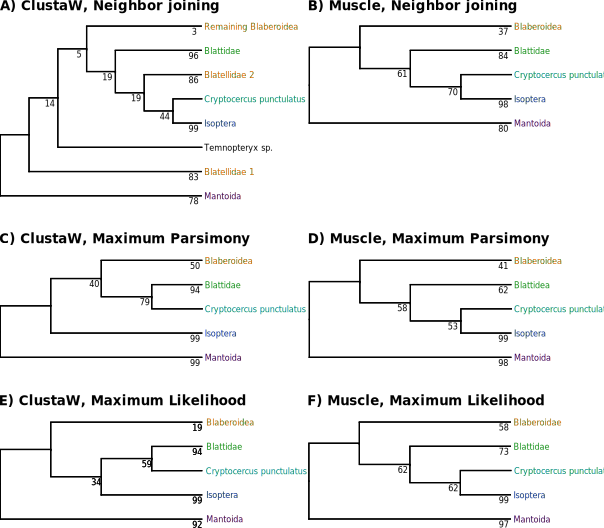
\includegraphics[scale=1]{images/collapsed_trees.pdf}
    \vspace{0.5cm}
    \mycaption{Bold short title}{of an example figure \lipsum[2].} 
    \label{fig:majortaxa}
\end{figure}

\section{Discussion}
  \label{chap:discussion}
  \begin{multicols}{2}
    \lipsum[1]
\end{multicols}

\begin{figure}[ht]
    \centering
    
\includegraphics[scale=0.9]{images/inward_small.pdf}
    \vspace{0.5cm}
    \mycaption{A fancy tree}{ \lipsum[1]}
    \label{fig:inward1}
\end{figure}

\begin{multicols}{2}
    \lipsum[1-6]
\end{multicols}

\section{Summary}
  \label{chap:summary}
  \input{chapters/summary.tex}

\pagebreak
\printbibliography

\pagebreak
\section{Appendix}
  \label{chap:appendix}
  \begin{figure}[H]
    \centering
    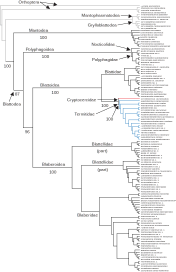
\includegraphics[scale=0.7]{images/inward_phyl.pdf}
    \vspace{0.5cm}
    \mycaption{Topology of Bayesian majority rules consensus tree of 2501 trees from \citet{inwardDeathOrderComprehensive2007}}{Red branch indicates position of \textit{Cryptocercus}, blue branches indicate termite lineage. Numbers under the branches indicate posterior probabilities (i.e. the proportion of the 2501 sampled trees that contain the node) for key nodes. Names of major clades (e.g superfamilies) are provisional.}
\end{figure}

\pagebreak
\begin{figure}[H]
    \centering
    \includegraphics[scale=0.9]{images/evangelista2019.pdf}
    \vspace{0.5cm}
    \mycaption{Time-calibrated phylogeny of Blattodea from \citet{evangelistaIntegrativePhylogenomicApproach2019}.}{Topology obtained from ML analysis of the decisive amino acid (aa) dataset (585 040 aa positions). Coloured circles represent BS support. Node dates (posterior mean) were inferred using the decisive aa dataset reduced to sites containing 95\% or more data completeness, and nine
    exhaustively vetted fossil calibrations. Error bars represent 95\% confidence intervals. Fossils used for calibrations indicated as numbers in black circles are: 1: \textit{Cretaholocompsa montespan}; 2: \textit{Archeorhinotermes rossi}; 3: \textit{Valditermes brenanae}; 4: \textit{‘Gyna’ obesa}; 5: \textit{Qilianiblatta namurensis}; 6: \textit{Juramantophasma sinica}; 7: \textit{Alexarasnia rossica}; 8: \textit{Raphogla rubra}; 9: \textit{Protelytron permianum}.}
    \label{fig:evangelista}
\end{figure}

\pagebreak
\csvreader[
longtable=lllll,
table head=
    \mycaption{A very long but beautiful table}{for the analysis with respective \textsc{GenBank}-ID's.} \label{tab:species}\\
    \toprule \bfseries No &\bfseries Order &\bfseries Family &\bfseries Species &\bfseries GenBankID \\ \midrule\endfirsthead\\ 
    \toprule \bfseries No &\bfseries Order &\bfseries Family &\bfseries Species &\bfseries GenBankID \\ \midrule\endhead \bottomrule\endfoot,
late after line=\\,
before reading={\catcode`\#=12},
after reading={\catcode`\#=6},
]{appendix/species.csv}{1=\No,2=\Order,3=\Family,4=\Species, 5=\GenBankID}{\No & \Order & \Family & \Species & \GenBankID}


% Append pdf outputs from other programs to the document
\includepdf[pages=-]{appendix/ab.pdf}
\includepdf[pages=-]{appendix/cd.pdf}
\includepdf[pages=-]{appendix/ef.pdf}

\end{document}
